\section{Synteny}

\subsection{Introduction}

\subsection{Methods}

\subsubsection{Generation of Dot Plots for Macrosynteny}

The workflow in Figure~\ref{fig:synteny-workflow} describes a process for preparing the dot plots for qualitative analysis of synteny.  Since synteny is the comparison of the order in which genes appear in the genome, the first step is to build data structures containing the gene names and positions along each scaffold.  We ignore the actual contents of the genes.

In the second step, we map identifiers of orthologous genes to common symbolic names so that genes can be cross-referenced between the genomes of different organisms. The mapping is accomplished by cross-referencing the gene IDs with the OrthoDB database.  
For each group of orthologous genes, OrthoDB provides the gene IDs for each gene from each organism and a unique group ID. Since synteny requires that each gene must have an ortholog in another genome, if a gene does not appear in OrthoDB, we exclude the gene from our analysis. 

\textcolor{red}{TODO: since we aren't using pathgroups we should allow 1-to-many orthologs now}

In the third step, we remove genes that appear in OrthoDB but do not have any orthologs in the other genomes involved in the comparison.

In the fourth step, we order the genes by their positions in the scaffolds.  We order the scaffolds arbitrarily.

In the last step, we produce a scatter plot.  The axes correspond to the ordered genes from each genome.  Markers indicate the presence of orthologous genes.  The formation of diagonal lines from multiple markers in a row indicate the presence of synteny.

\begin{figure}[H]
  \centering
  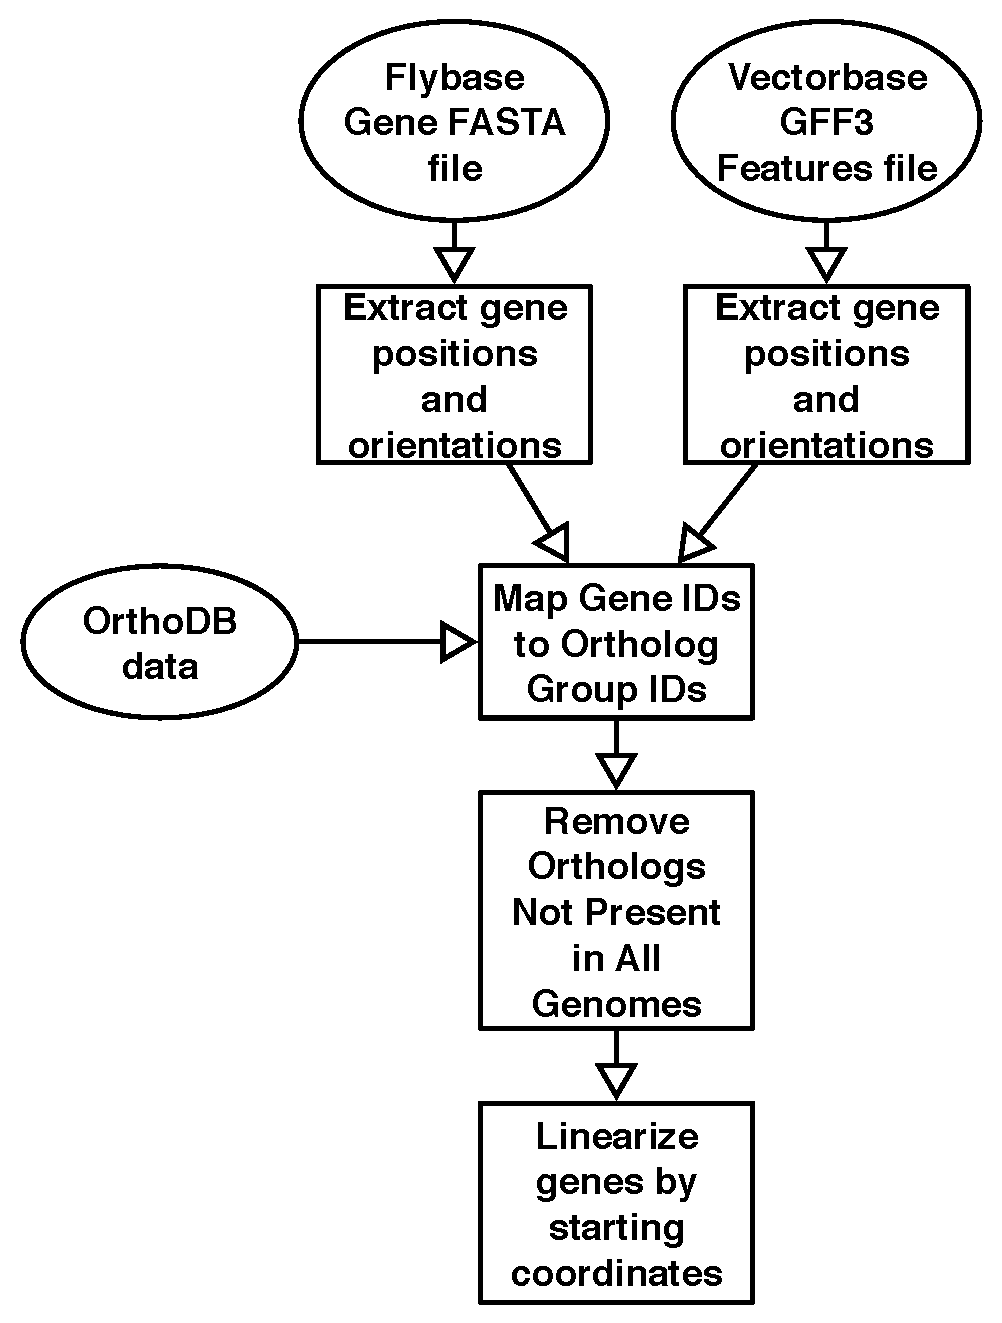
\includegraphics[width=0.5\textwidth]{figures/synteny/orthodb_dotplot_workflow}
  \caption{Workflow for Synteny}
  \label{fig:synteny-workflow}
\end{figure}

\subsubsection{Microsynteny}
\textcolor{red}{Synchro}

\subsection{Results}

\subsubsection{Genome Assembly Analysis}

\begin{figure}[H]
  \centering
  \begin{subfigure}[b]{0.45\textwidth}
    \includegraphics[width=\textwidth]{figures/synteny/genome_size_genes.pdf}
    \caption{Genome Sizes (Genes)}
  \end{subfigure}
  ~
  \begin{subfigure}[b]{0.45\textwidth}
    \includegraphics[width=\textwidth]{figures/synteny/scaffold_counts.pdf}
    \caption{Number of Scaffolds}
  \end{subfigure}
  ~
  \begin{subfigure}[b]{0.45\textwidth}
    \includegraphics[width=\textwidth]{figures/synteny/top5_scaffold_sizes.pdf}
    \caption{Top 5 Scaffold Sizes (Genes)}
  \end{subfigure}
  ~
  \begin{subfigure}[b]{0.45\textwidth}
    \includegraphics[width=\textwidth]{figures/synteny/gene_scaffold_cdf.pdf}
    \caption{Scaffold Genes CDF}
  \end{subfigure}
  \label{fig:scaffolds}
  \caption{}
\end{figure}

\subsubsection{\emph{L. longipalpis} vs. \emph{P. papatasi} Do Not Exhibit Macrosynteny}

\begin{figure}[H]
  \centering
  \begin{subfigure}[b]{0.45\textwidth}
    \includegraphics[width=\textwidth]{figures/synteny/papatasi_longipalpis_plot}
    \caption{\emph{L. longipalpis} vs. \emph{P. papatasi}}
  \end{subfigure}
  ~
  \begin{subfigure}[b]{0.45\textwidth}
    \includegraphics[width=\textwidth]{figures/synteny/dmel_dsim_plot}
    \caption{\emph{D. melanogaster} vs. \emph{D. simulans}}
  \end{subfigure}
  ~
  \begin{subfigure}[b]{0.45\textwidth}
    \includegraphics[width=\textwidth]{figures/synteny/aedes_anopheles_plot}
    \caption{\emph{Ae. aegypti} vs. \emph{A. gambiae}}
  \end{subfigure}
  ~
  \begin{subfigure}[b]{0.45\textwidth}
    \includegraphics[width=\textwidth]{figures/synteny/dmel_anopheles_plot}
    \caption{\emph{A. gambiae} vs. \emph{D. melanogaster}}
  \end{subfigure}
\label{fig:dot-plots}
\caption{}
\end{figure}

\subsubsection{Macrosynteny Requires Low Genome Assembly Fragmention and Evolutionary Conservation}

\begin{table}[H]
  \centering
  \begin{tabular}{|c|c|p{2.8cm}|c|} \hline
  Species & AUCs & Evolutionary Divergence (millions of years) & Macrosynteny \\ \hline
  \emph{L. longipalpis} vs. \emph{P. papatasi} & 0.896, 0.742 & & No \\ \hline
  \emph{D. melanogaster} vs. \emph{D. simulans} & 1.000, 0.990 & & Yes \\ \hline
  \emph{Ae. aegypti} vs. \emph{An. gambiae} & 0.922, 1.0 & & No \\ \hline
  \emph{D. melanogaster} vs. \emph{An. gambiae} & 1.0, 1.0 & & No \\ \hline
  \end{tabular}
  \caption{}
  \label{tab:synteny-species}
\end{table}

\subsubsection{\emph{L. longipalpis} vs. \emph{P. papatasi} Exhibit Microsynteny}

\textcolor{red}{block size distributions}

\textcolor{red}{analysis of individual blocks}

\subsubsection{\emph{L. longipalpis} vs. \emph{P. papatasi} Microsynteny Consists of Generic Housekeeping Genes}

\subsection{Discussion and Conclusion}